\documentclass[a4paper,11pt,fleqn]{article}%fleqn pour aligner les equations à gauche
\usepackage{../../Styles/Exercice}

\newcommand{\chnum}{Chapitre 1}
\newcommand{\chtitle}{Éléments dans l'Univers}
\newcommand{\dtype}{Exercices}



\begin{document}
\maketitle

\begin{multicols}{2}
\section{Réaction triple alpha}
Une des réactions qui se produit dans les étoiles est la réaction "triple alpha", qui est à l'origine de la formation des noyaux de carbone 12. Cette réaction se produit vers la fin de vie d'une étoile, quand la température (\SI{100}{\mega\kelvin}) devient suffisamment élevée pour que le béryllium 8 puisse rencontrer un noyau d'hélium et former le carbone 12 très stable.

%\begin{figure}[h!]
%\centering
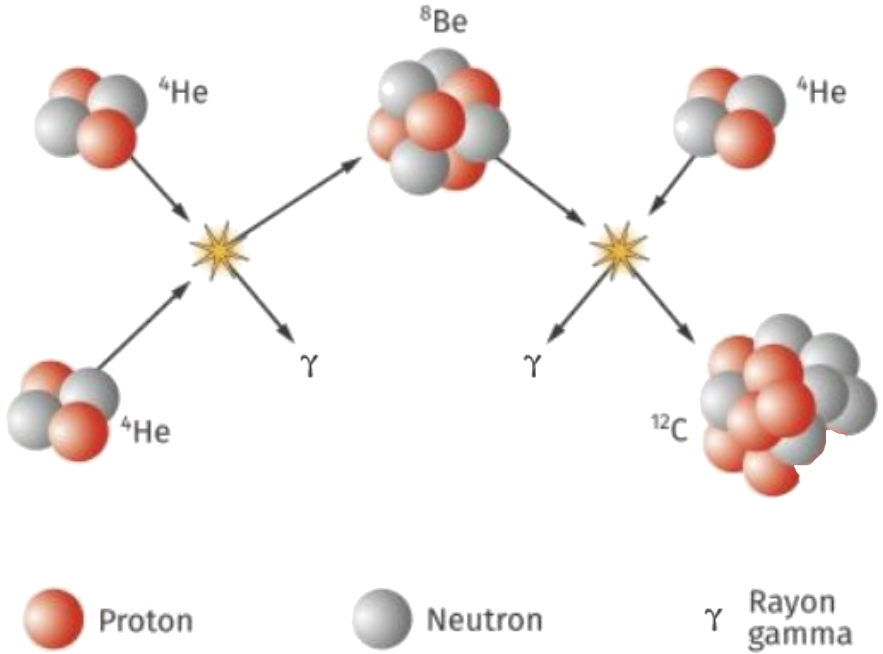
\includegraphics{Ressources/Act2_Fig1.png}
%\end{figure}

\textbf{Questions :}
\begin{enumerate}
	\item Donner la composition du noyau d'hélium 4 ($Z_{He}$ = 2), du béryllium 8 ($Z_{Be}$ = 4) et du carbone 12 ($Z_C$ = 6).
	\item Écrire les deux équations des réactions qui permettent de transformer l'hélium 4 en carbone 12.
	\item Indiquer de quel type de réaction il s'agit.
\end{enumerate}

\section{Abondance des éléments dans la croûte terrestre}
La croûte terrestre est une enveloppe superficielle d'une épaisseur moyenne de 6 (océans) à \SI{35}{km} (continents).\\
\begin{scriptsize}
\begin{tabular}{|>{\centering}m{1.5cm}|>{\centering}m{1.2cm}|>{\centering}m{1cm}|>{\centering}m{.8cm}|>{\centering}m{1.3cm}|>{\centering\arraybackslash}m{1.2cm}|} \hline
\textbf{Numéro atomique $Z$}& \textbf{1} & \textbf{8} & \textbf{11} & \textbf{12} & \textbf{13} \\ \hline
Symbole & H & O & Na & Mg & Al \\ \hline
Élément & Hydrogène & Oxygène & Sodium & Magnésium & Aluminium\\ \hline
Concentration (\unit{\milli\gram\per\kilo\gram}) & \num{1400} & \num{461000} & \num{28300} & \num{20900} & \num{81300}\\ \hline
\end{tabular}

\noindent
\begin{tabular}{|>{\centering}m{1.5cm}|>{\centering}m{1cm}|>{\centering}m{1.2cm}|>{\centering}m{.8cm}|>{\centering}m{1.3cm}|>{\centering\arraybackslash}m{1.2cm}|} \hline
\textbf{Numéro atomique $Z$} & \textbf{14} & \textbf{19} & \textbf{20} & \textbf{22} & \textbf{26}\\ \hline
Symbole & Si & K & Ca & Ti & Fe\\ \hline
Élément & Silicium & Potassium & Calcium & Titane & Fer\\ \hline
Concentration (\unit{\milli\gram\per\kilo\gram}) & \num{277000} & \num{26000} & \num{36300} & \num{4400} & \num{50000}\\ \hline
\end{tabular}
\end{scriptsize}

\textbf{Questions :}
\begin{enumerate}
	\item Identifier les trois éléments chimiques majoritaires dans la croûte terrestre.
	\item Réaliser un diagramme circulaire donnant la répartition des 10 éléments chimiques en considérant que ce sont les seuls présents dans la croûte terrestre.
	\item Comment ces éléments chimiques sont-ils arrivés sur Terre ?
\end{enumerate}

\section{La chaîne proton-proton}
Dans les étoiles, la fusion de quatre protons permet la formation de l'hélium 4. La chaîne "proton-proton" montre comment on passe de l'atome d'hydrogène à l'atome d'hélium. Cette réaction ne peut avoir lieu que lorsque la température dépasse le million de kelvins, pour vaincre la barrière coulombienne, qui résulte de la répulsion entre deux protons. \emph{Le noyau d'hydrogène contient un proton. On peut le représenter par "p" ou par l'écriture du noyau de l'atome d'hydrogène.}

\textbf{Questions :}
\begin{enumerate}
	\item Au cours de la première étape, deux protons fusionnent pour former du deutérium, un isotope de l'hydrogène contenant deux nucléons. Donner la composition du noyau de deutérium, puis éviter l'équation de la réaction. Identifier la particule émise au cours de cette réaction.
	\item Au cours de la deuxième étape, un proton fusionne avec un noyau de deutérium pour former un noyau d'hélium 3. Écrire l'équation de la réaction.
	\item Au cours de la dernière étape, deux noyaux d'hélium 3 réagissent pour former le noyau d'hélium 4 en libérant deux protons. Écrire l'équation de la réaction.
	\item Écrire l'équation de la réaction globale.
\end{enumerate}

\section{Lecture d'une courbe de décroissance}
Le 11 mars 2011, un accident majeur à la centrale de Fukushima (Japon) d'est produit à la suite d'une tremblement de terre suivi d'un tsunami. Les réacteurs ont rejeté plusieurs isotopes  radioactifs, dont ceux de l'iode. on mesure leur activité, proportionnelle au nombre d'atome.\\

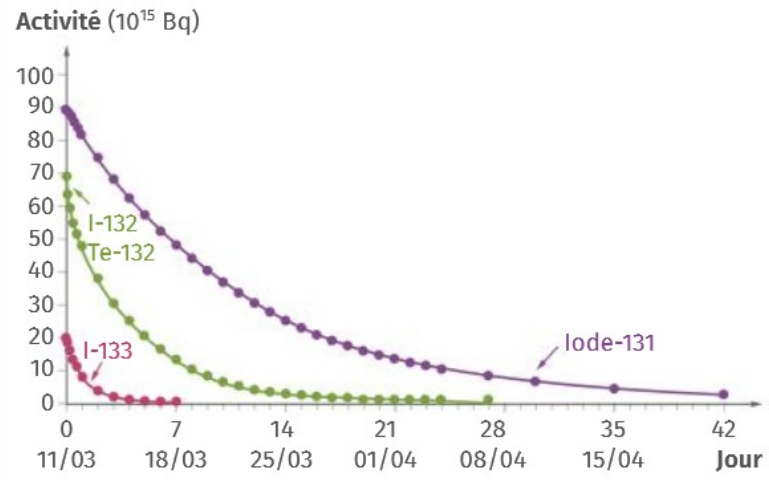
\includegraphics[scale=.3]{Ressources/Act2_Fig2.png}

\textbf{Questions :}
\begin{enumerate}
	\item Déterminer l'activité des isotopes I-131 et I-133 de l'iode et celle du tellure Te-132.
	\item Déterminer la demi-vie de chacun de ces éléments.
	\item Déterminer, pour chaque élément, la durée au bout de laquelle l'activité est inférieure à \SI{10}{\percent} de l'activité initiale.
\end{enumerate}

\section{Datation au carbone 14}
Un morceau de charbon a été retrouvé à l'entrée d'une grotte et on le soumet à une datation au carbone 14. Cet élément radioactif est présent dans tout être vivant à un taux constant. À leur mort, les échanges de matière avec le milieu n'ayant plus lieu, le taux de carbone 14 diminue car il se désintègre. La mesure de ce taux dans un échantillon permet donc de dater approximativement sa mort.\\
\textbf{Donnée :} La demi-vie du carbone 14 est de $t_{1/2}$ = \SI{5734}{ans}.\\
Déterminer l'âge du morceau de charbon sachant que l'activité de l'échantillon testé montre que le nombre d'atomes de carbone 14 est 16 fois plus faible qu'à sa formation.

\section{Datation des roches lunaires : mission Apollo XI}
Lors de la mission Apollo XI, les astronautes ont rapporté des pierres lunaires recueillies sur la mer de la Tranquillité. Une des méthodes utilisées pour dater les roches lunaires est basée sur le couple \ce{^{40}K}/\ce{^{40}Ar} (potassium/argon).\\
Dans un échantillon de \SI{1}{g} on a mesuré les quantités de \ce{^{40}K} (\SI{2,93}{\micro\gram}) et de \ce{^{40}Ar} (\SI{82E4}{\centi\meter\cubed}) qui est retenu par la riche bien qu'il soit à l'état gazeux. Soit en nombre d'atome : $N_K(t)$ = \num{4,41E16} et $N_{Ar}(t)$ = \num{2,06E17}.\\

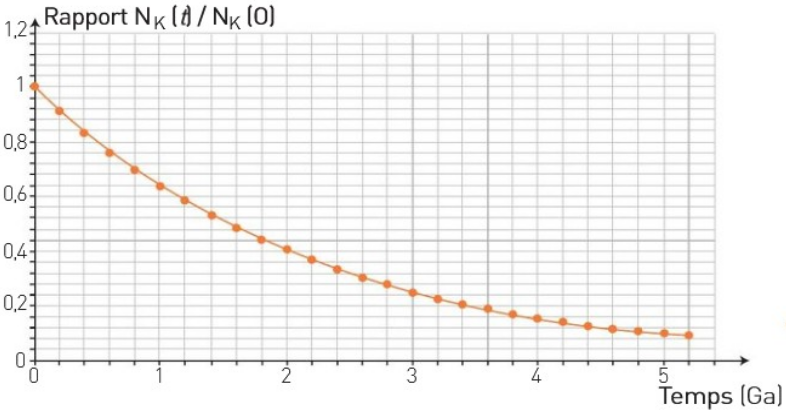
\includegraphics[scale=.35]{Ressources/Act2_Fig3.png}

\begin{enumerate}
	\item Indiquer si la réaction nucléaire suivante est une désintégration ou une fusion. $$\ce{^{40}_{19}K -> ^{40}_{18}Ar + ^{0}_{1}e+}$$
	\item Déduire le nombre initial d'atomes de potassium : $N_K(0)$ puis le rapport $N_K(t)$/$N_K(0)$.
	\item En déduire l'âge de l'échantillon. Comparer cette donnée à l'âge de la Terre.
\end{enumerate}

\section{La conservation radioactive des aliments}
L'irradiation à faible dose des fruits et légumes par le cobalt 60 (\ce{^{60}Co}), dont la demi-vie est 5 ans, permet de prolonger leur durée de conservation en éliminant parasites et insectes.
\begin{enumerate}
	\item Recopier et compléter le tableau suivant.
	avec $N$ le nombre de noyaux restants.
\end{enumerate}
	\begin{scriptsize}
	\begin{tabular}{|>{\centering}m{1cm}|>{\centering}m{.8cm}|>{\centering}m{.8cm}|>{\centering}m{.8cm}|>{\centering}m{.8cm}|>{\centering}m{.8cm}|>{\centering\arraybackslash}m{.8cm}|} \hline
	\textbf{t} (ans) & 0 & 5 & 10 & 15 & 20 & 25\\ \hline
	\textbf{N} & 8000 & & & & & \\ \hline
	\end{tabular}
	\end{scriptsize}
	
\begin{enumerate}[resume]
	\item Tracer la courbe $N = f(t)$.\\
	Échelles : \SI{1}{cm} pour 2 ans et \SI{1}{cm} pour \num{1000} noyaux en ordonnée.
	\item Déterminer graphiquement la durée au bout de laquelle il ne reste qu'un cinquième du nombre initial des noyaux.
\end{enumerate}
\end{multicols}



\end{document}